%%!TeX program = xelatex
%% 부득이하게 pdflatex을 사용해야 할 경우 위의 magic comment를 제거하십시오.

% Initiated by 정민석(2014년도 경기과학고 수학과전문교원)
% Continously being modified by 경기과학고 TeX 사용자협회
% Website : http://gshslatexintro.github.io 

\documentclass{gshs_report}
% 아래의 함수를 사용하면 이미지 파일들을 같은 디렉토리 내에 images 라는 이름을 가진 폴더를 생성한 후, 그 폴더 안에 넣어 사용할 수 있습니다.
% 사용하고자 한다면 주석을 푸십시오.
\graphicspath{{images/}}
% 이곳에 필요한 별도의 패키지들을 적어넣으시오.
%\usepackage{...}
\usepackage{verbatim} % for commment, verbatim environment
\usepackage{spverbatim} % automatic linebreak verbatim environment
%\usepacakge{indentfirst}
\usepackage{tikz}
%\tikzset{
%	image label/.style={
%		every node/.style={
			%fill=black,
			%text=white,
%			font=\sffamily\scriptsize,
%			anchor=south west,
%			xshift=0,
%			yshift=0,
%			at={(0,0)}
%		}
%	}
%}
\usepackage{amsmath}
\usepackage{amsfonts}
\usepackage{amssymb}
\usepackage{float}
\usepackage{graphicx}
\usepackage{tabularx}
\usepackage{multirow}
\usepackage{booktabs}
\usepackage{longtable}
\usepackage{gensymb}
%\usepackage{subcaption}
%\usepackage{floatrow}
%\usepackage{pict2e}
%\usepackage[backend=biber,style=authoryear]{biblatex}
%\usepackage{biblatex}
\usepackage{pgfplots}
\pgfplotsset{
	compat=newest,
	label style={font=\sffamily\scriptsize},
	ticklabel style={font=\sffamily\scriptsize},
	legend style={font=\sffamily\tiny},
	major tick length=0.1cm,
	minor tick length=0.05cm,
	every x tick/.style={black},
}

\usetikzlibrary{shapes}
\usetikzlibrary{plotmarks}
\usepackage{listings}
\usepackage{hologo}
\usepackage{makecell}

\lstset{
	basicstyle=\small\ttfamily,
	columns=flexible,
	breaklines=true
}

\citation

\bibdata

%: ----------------------------------------------------------------------
%:               보고서 정보를 입력하시오
% ----------------------------------------------------------------------
% 아래와 같은 command를 만들면 길이가 긴 용어를 간편하게 사용할 수 있습니다. 단, 이미 지정된 함수명들은 새로운 함수명으로 사용할 수 없습니다.
\newcommand{\gshs}{Gyeonggi Science High School for the Gifted }

\researchtype{기초} % 기초 / 심화
\reporttype{결과} % 중간 / 결과

\title{보고서 제목} % 제목 개행 시 \linebreak 사용. \\나 \newline 은 안됨.
\englishtitle{English title}% 제목 개행 시 \linebreak 사용. \\나 \newline 은 안됨.

\author[1] {홍길동} % 제 1 저자명
\email[1]{hong@e-mail.address} % 제 1 저자 이메일
\author[2] {전우치} % 제 2 저자명
\email[2]{cheon@e-mail.address} % 제 2 저자 이메일
\advisor{박기현} % 지도교사명
\advisorEmail{guitar79@gs.hs.kr} % 지도교사 이메일

%%%%%%%%%%%%%%%%%%%%%%%%%%%%%%%%%%%%%%%%%%%%%%%
%%%% researchtype이 '심화'일 경우에만 나타남 %%%%
\professor{교수님} % 지도교수명
\professorEmail{professor@e-mail.address} % 지도교수 이메일
%%%%%%%%%%%%%%%%%%%%%%%%%%%%%%%%%%%%%%%%%%%%%%%%
\summitdate{2018}{02}{07} % 제출일 (연, 월, 일)
\newtheorem{definition}{정의}
 % usepackage 등의 명령어는 여기에.
\usepackage{cite}
\usepackage{textcomp}
\usepackage{tocloft}
\setlength{\cftbeforesecskip}{0pt}
\setlength{\cftbeforesubsecskip}{0pt}
\setlength{\cftbeforesubsubsecskip}{0pt}

% 본문 시작
\begin{document}

%표지만들기
%makecover 함수와 관련하여 "Underfull \hbox (badness 10000) in paragraph" 오류는 무시하십시오. (TeXstudio ver 2.9.4 오류 기준)
%\makecover

%초록(영문)
%\maketitle  % command to print the title page with above variables
\makecover  % command to print the title page with above variables

\setcounter{page}{1}
\renewcommand{\thepage}{\roman{page}}

%----------------------------------------------
%   Table of Contents (자동 작성됨)
%----------------------------------------------
\cleardoublepage
\addcontentsline{toc}{section}{Contents}
\setcounter{secnumdepth}{3} % organisational level that receives a numbers
\setcounter{tocdepth}{3}    % print table of contents for level 3
\baselineskip=2.2em
\tableofcontents


%----------------------------------------------
%     List of Figures/Tables (자동 작성됨)
%----------------------------------------------
\cleardoublepage
\clearpage
\listoffigures	% 그림 목록과 캡션을 출력한다. 만약 논문에 그림이 없다면 이 줄의 맨 앞에 %기호를 넣어서 코멘트 처리한다.

\cleardoublepage
\clearpage
\listoftables  % 표 목록과 캡션을 출력한다. 만약 논문에 표가 없다면 이 줄의 맨 앞에 %기호를 넣어서 코멘트 처리한다.


\cleardoublepage
\clearpage

%---------------------------------------------------------------------
%                  영문 초록을 입력하시오
%---------------------------------------------------------------------
%\begin{abstracts}     %this creates the heading for the abstract page
%	\addcontentsline{toc}{section}{Abstract}  %%% TOC에 표시
%	\noindent{
%			Put your abstract here. Once upon a time, \gshs said : `The first, and the best.'
%	}
%\end{abstracts}

%\cleardoublepage
%\clearpage

\begin{abstractskor}
	\addcontentsline{toc}{section}{초록}  %%% TOC에 표시
	\noindent{
본 논문에서는 초점 조절 구동 시스템을 구현하는 방법을 제안한다. 초점 조절 구동 펌웨어는 기본적으로 Arduino를 사용하며 여러 기능이 존재하여 자유로운 설정이 가능하다. ASCOM 드라이버는 C\# 코딩을 이용하여 컴퓨터로 정보 전달이 가능하다. 본 논문에서 제안된 방법은 사람이 손으로 제어하는 것보다 정밀하고 빠르게 천체망원경의 초점을 맞출 수 있도록 편의성을 제공하기 위한 바탕 역할을 할 수 있다.
	}
\end{abstractskor}






 % Abstract

%%%%%%%%%%%%%%%%%%%%%%%%%%%%%%%%%%%%%%%%%%%%%%%%%%%%%%%%%%%
%%%% Main Document %%%%%%%%%%%%%%%%%%%%%%%%%%%%%%%%%%%%%%%%
%%%%%%%%%%%%%%%%%%%%%%%%%%%%%%%%%%%%%%%%%%%%%%%%%%%%%%%%%%%
\cleardoublepage
\clearpage
\renewcommand{\thepage}{\arabic{page}}
\setcounter{page}{1}

%각 장을 아래와 같이 sub 폴더 안에 만들어서 넣으면 편리하다.
\section{서론}

\subsection{연구의 필요성}

천체를 관측할 때 초점을 맞춘다면 관측할 천체의 모습이 더 선명하게 보인다. 일반적으로 대부분 망원경은 초점을 손으로 맞출 수 있게 설계되어있다. 천체망원경으로 사진 관측을 할 때 정확한 초점 조절은 사진의 품질에 영향을 미치는 요소 중의 하나이다. 초점 조정 시 어려운 점은 초점을 조정하기 위해 초점 조절 노브에 손이 닿으면 진동이 발생하고, 그 진동이 사진의 품질에 영향을 준다. 또한, 초점을 조절할 때 손으로 돌리는 것은 미세한 조정에는 어려움이 있다. 또한, 초점이 완벽하게 맞지 않았는데도 이러한 사진을 찍기 위해서 초점을 맞추는데 많은 시간을 투자해야 한다. 이렇듯 사진을 통하여 정밀한 천체의 사진이 필요한 경우 사람의 손으로는 무리가 있다. 하지만 모터 초점 조절 장치가 있다면 손으로 초점을 맞추는 것보다 정확하게 초점을 맞출 수 있게 된다. 
\begin{figure}[h]
	\begin{subfigure}{0.5\textwidth}
		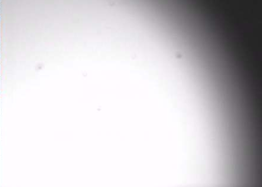
\includegraphics[width=0.9\linewidth, height=5cm]{before} 
		\caption{초점 맞추기 전}
		\label{fig:before}
	\end{subfigure}
	\begin{subfigure}{0.5\textwidth}
		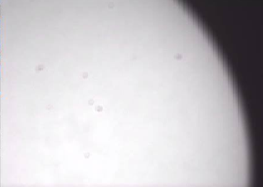
\includegraphics[width=0.9\linewidth, height=5cm]{after}
		\caption{초점 맞춘 후}
		\label{fig:after}
	\end{subfigure}
	\caption{초점을 맞추기 전과 후 비교}
	\label{fig:image1}
\end{figure}
Fig 1.(a), Fig 2.(b)에서 알 수 있듯이 모터 초점 조절 장치를 이용하여 초점을 맞추면 아무것도 하지 않고 그냥 관측했을 때에 비해서 훨씬 정확하게 천체를 관측할 수 있게 된다. Fig 1.(a)와 Fig 2.(b)를 비교하여 보면 Fig 2.(b)의 표면이 훨씬 더 선명하다는 사실을 알 수 있다. 하지만, 모터를 이용하여 초점을 맞춘다고 해도 우리 눈으로 초점을 맞추는 것이기 때문에 정확하지 않을 수 있다. 이러한 문제를 해결하기 위하여 만들어진 자동 초점 조절 장치가 있다. 자동 초점 조절 장치가 현재 개발된 제품이 미국 Starizona 회사의 Micro Touch이다. 이 제품은 자동 초점 조절 시스템이 구현이 잘 되어 있으나, 가격이 499달러로 부담 이 있을 수 있다. 또한, 실제로 모터 초점 조절 장치와 연계해 초점을 맞춰주는 다른 Software도 몇 종류가 있으나 오류가 발생하는 경우가 있다. 따라서 천체망원경의 모터 초점 조절 장치의 컨트롤러 구동 시스템을 개발하면 여러 천체를 관측하는 데 있어서 보다 정확한 사진들을 얻을 수 있을 것이다.

%\begin{wrapfigure}{l}{0.3\textwidth}
%	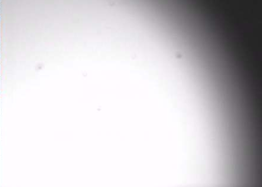
\includegraphics[width=1\linewidth]{before}
%	\caption{초점 맞추기 전}
%	\label{fig:before}
%\end{wrapfigure}

\subsection{연구목적}

본 논문에서 제안된 방법은 사람이 손으로 제어하는 것보다 정밀하고 빠르게 천체망원경의 초점을 맞출 수 있도록 편의성을 제공하기 위한 기반을 제공하기 위함이다. 이 연구는 Arduino를 이용하여 천체망원경을 이용한 천체관측을 시행할 때 필요한 모터 초점 조절 장치를 조정할 수 있는 모터 초점 조절 장치 컨트롤러 구동 시스템을 구현하고, 초점을 조정하는 알고리즘을 만들어서 천체의 초점을 맞출 수 있도록 한다. 그리고 이와 통신을 할 수 있는 시스템도 개발하여 편의성을 늘리고, ASCOM 드라이버를 제작하여 컴퓨터와의 통신을 가능하게 하는 것이 이 연구의 목표이다. % body1
\section{이론적 배경}

\subsection{Micro Touch와 모터의 조절}

그림3 이 바로 Micro Touch로, 시중에 나와 있는 모터 초점 조절 장치이다. 이를 옆의 컴퓨터와 연결하여 컴퓨터에서도 ASCOM이라는 프로그램을 이용하여 원격으로 모터의 초점을 맞출 수 있도록 설정할 
\begin{wrapfigure}{l}{0.25\textwidth}
	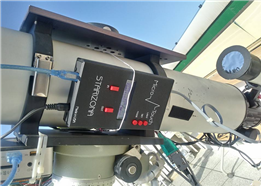
\includegraphics[width=1\linewidth]{telescope1}
	\caption{Micro Touch가 달린 천체망원경}
	\label{fig:telescope1}
\end{wrapfigure}
수가 있다. Fig.2에서 나온 위의 두 버튼(IN, OUT)은 각각 초점을 맞추기 위해 망원경의 길이를 줄이거나 늘일 수 있는 버튼이다. Micro Touch를 수동 혹은 자동으로 작동시켜 IN 또는 OUT의 명령을 내렸을 경우, 모터 초점 조절 장치가 작동하게 된다. 이 모터 초점 조절 장치는 모터를 움직여 천체망원경의 경통의 길이를 조절할 수 있도록 한다. 경통의 길이가 변화하면 그에 따라서 빛이 퍼지는 정도가 달라지므로 이를 잘 조정하면 망원경으로 관측하는 천체의 초점을 맞출 수 있다.

\subsection{온습도 감지기를 이용한 온도 및 습도의 조절}

\begin{wrapfigure}{l}{0.05\textwidth}
	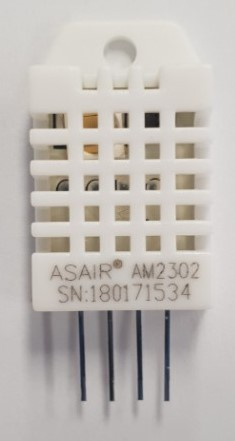
\includegraphics[width=1\linewidth]{DHT22}
	\caption{DHT22}
	\label{fig:DHT22}
\end{wrapfigure}
이 연구를 진행하는 데 Arduino를 사용하는 것이 가장 기본이라고 판단하였기 때문에 Arduino로 실행할 수 있는 것 중 쉬운 축이라고 생각되는 온습도 감지기(DHT22)를 활용하여 온습도를 측정하는 일이었다. 기판을 짜고 코드를 입력하면 Serial Monitor에 온도와 습도가 delay 함수에서 지정한 만큼의 간격을 두고 계속 출력된다. 이를 응용하여 OLED(OLED1306)에 온도와 습도를 실시간으로 출력하는 프로그램을 만들 수도 있다.

\subsection{스테핑 모터}

\subsubsection{스테핑 모터의 종류}

스테핑 모터의 종류는 크게 bipolar와 unipolar 타입으로 나눌 수 있다. 하나는 2상 6선식이라고 불리는 bipolar 스테핑 모터로, 전선이 6개가 연결되어 있다. 2상 4선식이라고도 불리는 unipolar 타입은 전선이 4개가 연결된 모터로, 구동 방식은 bipolar 타입과 크게 다르지 않다.\\
본 논문에서 사용된 스테핑 모터는 2상 6선식 모터이지만, 그 구동 방식이 비슷하므로 bipolar 스테핑 모터에서 필요 없는 2번 선과 5번 선을 제거하는 것으로 bipolar 스테핑 모터를 unipolar 스테핑 모터처럼 구동할 수 있다.

\subsubsection{스테핑 모터의 작동 원리}

\begin{wrapfigure}{l}{0.5\textwidth}
	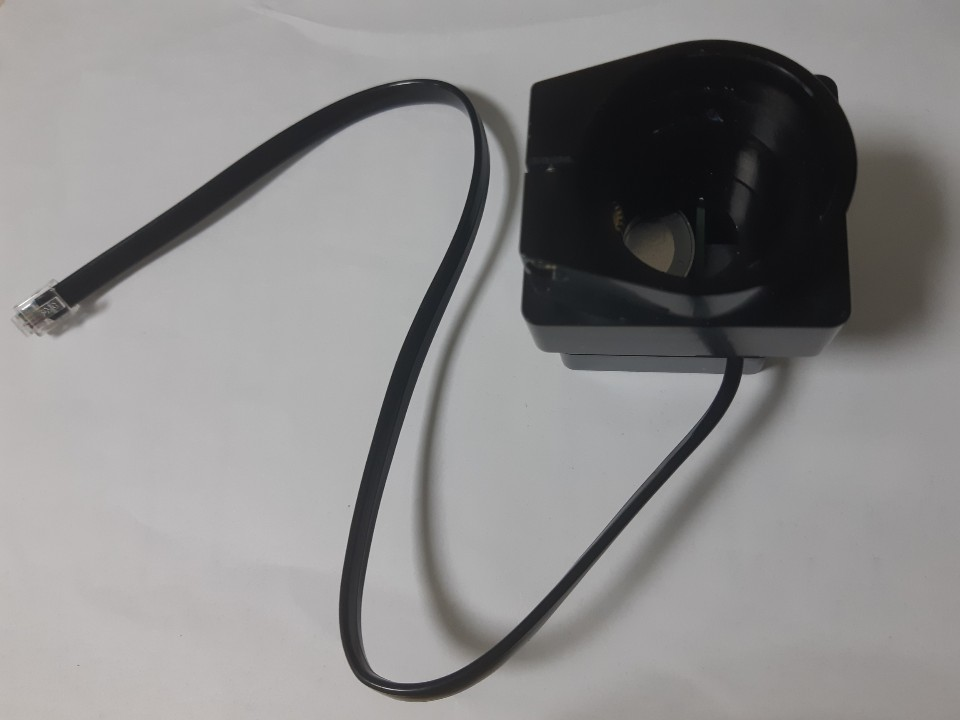
\includegraphics[width=1\linewidth]{stepmotor}
	\caption{스테핑 모터}
	\label{fig:stepmotor}
\end{wrapfigure}
우리가 실생활에서 볼 수 있는 모터 대부분은, 예를 들어 선풍기의 모터는, DC모터이다. DC모터는 전류가 흐르는 상태에서는 계속 회전하기 때문에 원하는 위치에서 멈추는 것이 어렵다. 하지만 스테핑 모터는 회전자 주위에 여러 고정자가 존재하여, 이 고정자들에 흐르는 전류의 변화량에 따라서 회전자 내부의 자석을 회전시키기 때문에, 전류의 양에 따라서 일정한 각도를 정확하게 회전시킬 수 있다. 따라서 본 연구와 같이 회전시키는 것이 중심이 아닌, 정확하게 얼마나 돌아갔는지(어느 각도만큼 돌아갔는지가 중요하게 작용할 때) 대부분 스테핑 모터를 활용하고는 한다. 이렇듯 선별로 흐르는 전류의 양에 의해 회전하는 정도와 속도를 결정할 수 있기에 흔히 ‘마이크로 스테핑’을 이용하여 전류를 여러 단계로 나누어 흘려보내어 더 정밀하게 모터를 제어하는 방법들도 존재한다. 대부분의 스테핑 모터는 1 스텝당(full step) 1.8도를 돈다고 알려져 있다.

\subsection{각 부품의 설명}

\subsubsection{Arduino ARDUINO NANO}

모터 초점 조절 장치 컨트롤러를 만드는 데 있어 가장 중요한 부품으로, 일종의 작은 컴퓨터와 같은 역할을 한다. Arduino는 마이크로 컨트롤러를 달고 있는 기판으로, Arduino의 여러 가지 핀에 전선을 연결한 뒤에 코딩하여 Arduino에 올리면 Arduino가 코딩된 내용을 그대로 실행할 수 있도록 하는 hardware이다. 내부에 컴퓨터 역할을 하는 MPU인 ATmega328가 탑재되어 있으며, 5V를 공급할 시에 작동한다. 크기는 45mm x 18mm이다.

\subsubsection{0.96" oled screen I2C}

Arduino와 I2C 방법으로 통신을 할 수 있는 OLED 스크린이다. 여러 가지 정보가 전달되며, 모터를 얼마나 돌릴 것인지, 혹은 얼마나 돌려져 있는지 등이 표현될 수 있다.

\subsubsection{DHT22}

온도와 습도를 측정할 수 있는 감지기로, -40~80℃의 넓은 온도 측정범위와 약 0.5℃밖에 없는 오차를 가지고 있다. 이를 통해 온도나, 렌즈의 온도 상태를 볼 수 있으며, 이를 사용하면 좀 더 정밀한 측정이 가능할 것이다.

\subsubsection{Apem MJTP1230B 버튼스위치}

누르는 버튼의 일종으로, 다리가 4개 달린 상태에서 같은 방향에 있는 2개의 전선이 연결된 방식의 버튼이다. 내부의 pull-up 저항을 활용하면 Arduino와 직접 연결하는 것으로 작동시킬 수 있다.

\subsubsection{BP5277-90}

모터를 돌리기 위해서는 12V의 전압이 필요하다. 즉, 12V의 전압을 이용하여 모터를 돌리면서 Arduino를 실행시키기 위해서는 12V를 Arduino의 입력전압인 5V까지 낮출 필요가 있다. 이에 regulator와 축전기를 활용하여 가장 안전하게 5V까지 전압을 낮출 수 있는 regulator를 선택하였다.

\subsubsection{HC-06 bluetooth}

무선통신 장치이다. 여러 가지 무선통신 장치 중에서 블루투스 module의 역할을 하고 있다.

\subsubsection{LED 3mm 90', Ohmite OD473JE}

전원이 여러 개가 존재할 수 있으므로, 모터가 돌아갈 수 있는 전압인 12V의 외부전압이 들어왔을 때만 LED가 깜빡일 수 있게 하여 모터가 돌아갈 수 있는 전압이 되었는지 확인할 수 있도록 하는 역할을 하고 있다.

\subsubsection{Panasonic EEA-GA1C100H}

모터를 돌리는 상황에서 큰 전류를 사용하기 때문에 전류가 역방향으로 흐르는 등의 문제를 방지하기 위하여 100μF의 축전기를 사용하였다.

\subsubsection{SparkFun WRL-13678 (ESP8266, ESP01)}

무선통신 장치이다. 여러 가지 무선통신 장치 중에서 WIFI 모듈을 담당한다. 입력전압이 5V가 아닌 3.3V이다.

\subsubsection{Sprague 1C10X7R104K050B}

부품별로 각각 연결된 축전기로, 모두 같은 전압 차를 가지고 있지만, 전류의 noise filtering을 하는 역할로, 필수적으로 사용되었다.

\subsubsection{TMC2100 (DRV8825)}

스테핑 모터를 돌리는 데 있어서 전류를 쉽게 조절할 수 있게 해주는 module이다. 이뿐만이 아니라 모터를 좀 더 세밀하게 돌릴 수 있게 해주는(스텝 당 돌아가는 각도를 줄여주는) 마이크로 스텝을 구현 가능한데, DRV8825의 핀 중 M1, M2, M3의 up, down을 조절하여 full step을 원래 각도와 비교하면 얼마나 적게 돌릴 것인지 결정할 수 있게 한다. 본 모델은 최대 1/32까지의 마이크로 스텝이 가능하다.

\subsubsection{TE Connectivity/AMP 5525258-3 및 Wurth Elektronik 694106301002}

12V 외부전원과 모터를 연결하는 선을 연결할 수 있게 하는 module이다.

\subsection{사용한 망원경}

\begin{wrapfigure}{l}{0.14\textwidth}
	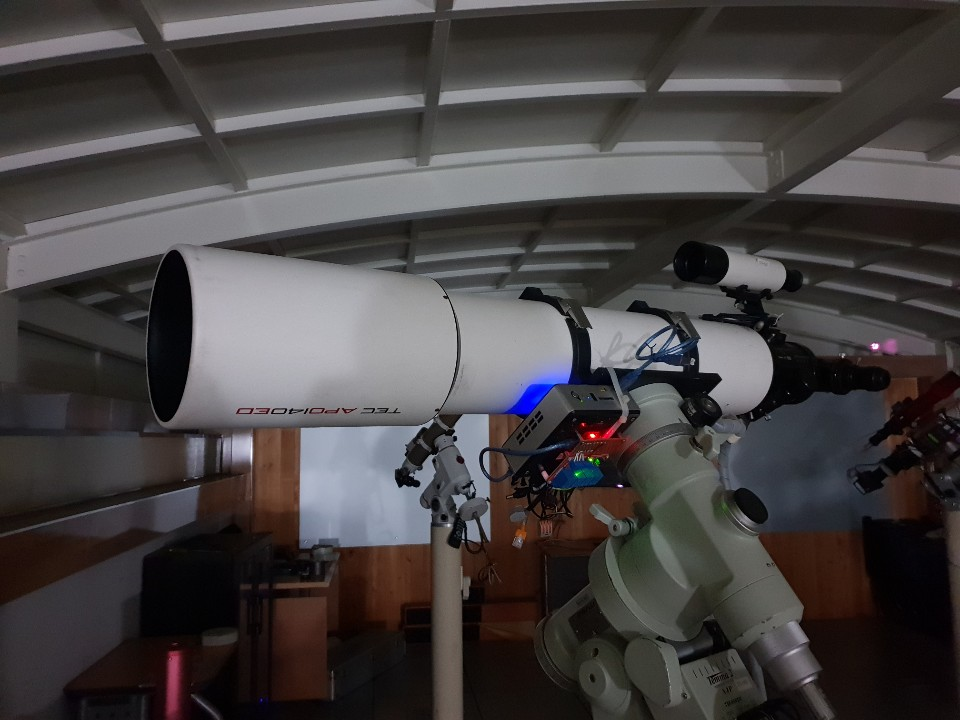
\includegraphics[width=1\linewidth]{telescope}
	\caption{사용한 망원경}
	\label{fig:telescope}
\end{wrapfigure}
TEC140 광학계에는 Starlight Instruments에서 제작한 3.5" Feather Touch Focuser가 장착되어 있다. Starlight Instruments에서는 3.5" Feather Touch Focuser에 장착할 수 있는 STEPPER MOTOR와 MICRO TOUCH FOCUSING SYSTEM을 제작하여 판매하고 있으며, 이 외에도 다른 망원경의 모터 초점 조절 장치에도 사용할 수 있도록 컨트롤러를 구현하는 것을 목표로 삼는다.

\subsection{자동초점조절 알고리즘 및 관련 논문 고찰}

이덕규 외(2014)는 복합재 광구조체와 결합하여 전자광학카메라의 영상 품질을 향상시킬 수 있는 초점 조절 장치를 개발하였다.\cite{leedukgu2014}\\
윤종환 외(2011)는 선명도에 관한 기울기를 이용하여 초점이 맞았는지를 확인하는 방법을 사용하였다.\cite{yunjonghwan2011lcd}\\
박석휘 외(2009)는 모바일 폰용 자동 초점 조절 알고리즘을 초점 값 계산 알고리즘을 이용하여 구현하였다.\cite{parksukhui2009Median}\\
이성희 외(1998)는 각 화소들의 미디언 값의 차이를 이용하여 초점을 맞추는 알고리즘을 구현하였다.\cite{leeseonghee1998Median}
 % 이론적 배경
\section{연구 과정}

\subsection{천체망원경 모터 초점 조절 장치 컨트롤러 제작}

\subsubsection{회로도 제작}

천체망원경 모터 초점 조절 장치 컨트롤러를 제작하기 위해서는 위에서 나열한 대로의 여러 가지 부품들이 필요할 것이다. 하지만 이러한 부품들의 개수가 많아질수록 회로도가 복잡한 정도는 기하급수적으로 늘어나기 때문에 여러 프로그램의 도움을 받아 회로도를 그리는 것이 일반적인 방법이다.
\begin{wrapfigure}{l}{0.5\textwidth}
	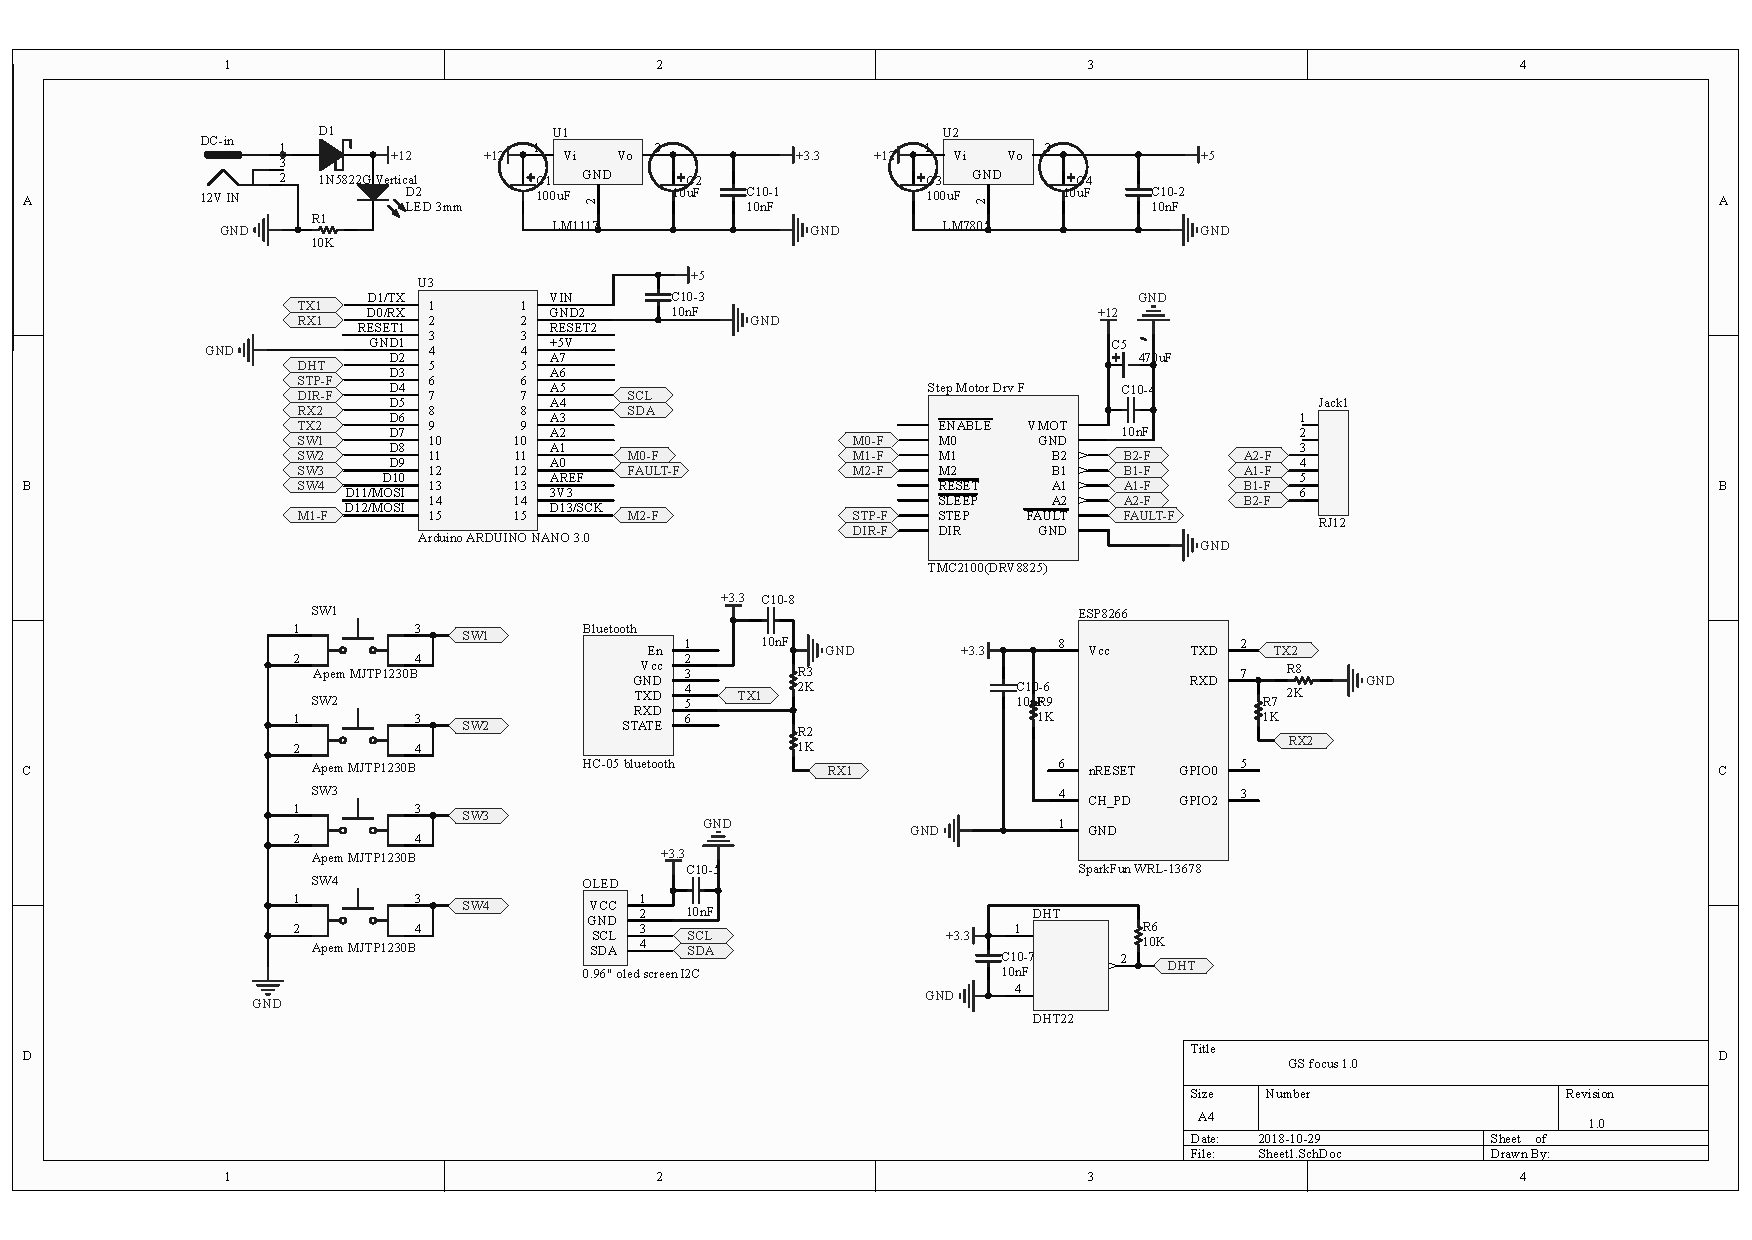
\includegraphics[width=1\linewidth]{Schematic_Prints}
	\caption{Circuitmaker를 이용하여 만든 차트}
	\label{fig:Schematic_Prints}
\end{wrapfigure}
생각보다 Circuitmaker 프로그램의 사용법을 숙지하는 데 오랜 시간이 걸렸기 때문에, 그사이에 진행된 연구에서는 만능기판에 여러 가지 부품들을 전선으로 연결하여 사용하는 방법을 택하였고, 연구가 진행되어 만능기판이 복잡해짐에 따라서 여러 프로그램의 도움을 받게 되었다.\\
연구 초기과정에서는 Arduino와 직접 연동이 가능한 ‘Fritzing’이라는 프로그램을 사용하였지만, 연구가 진행될수록 다른 부품들과 실제로 구현이 가능한 PCB 회로기판을 만들 수 있어야 했기 때문에 보편화한 PCB 회로제작 프로그램이면서 ‘협업’ 기능을 이용하여 동시에 수정이 가능한 ‘Circuitmaker’라는 프로그램을 사용하게 되었다.

\subsubsection{회로도 제작 시 주의 사항}

각 부품을 사용할 때에는 각 부품의 허용 전류와 같은 여러 가지 특징들을 생각하여 회로를 배선해야 한다. 예를 들어 WIFI 모듈인 ESP8266과 같은 경우 그 입력전압이 Arduino의 출력 전압인 5V가 아닌 3.3V이기 때문에 주의하여야 한다. 또한, 각 부품의 칩별로 제조한 회사의 data sheet를 참조하여 부품을 사용하면서 여러 가지 문제점들을 미리 방지하였다.\\
특히 5V를 3.3V로 바꾸는 과정에서는 전압 나눔 회로를 이용하여 전압을 나눌 수 있으나, 12V를 5V로 바꾸는 과정에서는 전류를 제어하는 것이 필요하므로 부득이하게 regulator를 사용하게 되었다.
\begin{figure}[h]
	\begin{subfigure}{0.5\textwidth}
		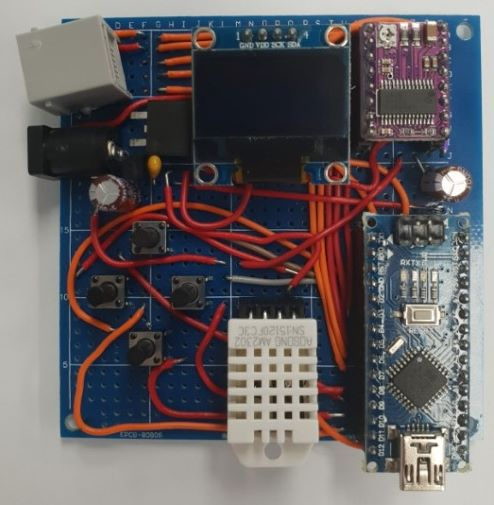
\includegraphics[width=0.9\linewidth, height=5cm]{circuit1} 
		\caption{만능기판으로 제작한 회로}
		\label{fig:circuit1}
	\end{subfigure}
	\begin{subfigure}{0.5\textwidth}
		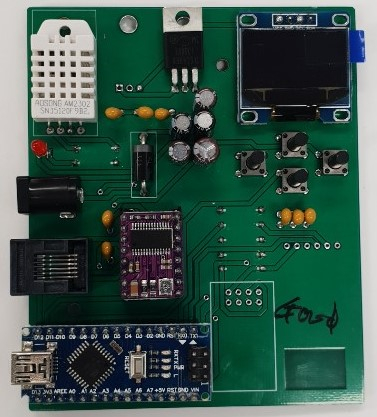
\includegraphics[width=0.9\linewidth, height=5cm]{pcbcircuit}
		\caption{PCB 기판으로 제작한 회로}
		\label{fig:pcbcircuit}
	\end{subfigure}
	\caption{제작한 회로도}
	\label{fig:image2}
\end{figure}

\subsubsection{펌웨어 개발}

Arduino를 이용하여 모터 초점 조절 장치를 만드는 데 필요한 기술들은 크게 4가지이다. 먼저, Arduino와 모터 드라이버(DRV8825)를 이용하여 모터를 돌릴 수 있어야 한다. 두 번째로, 스위치를 활용하여 모터의 움직임을 조절할 수 있게 하였다. 세 번째로, 모터를 조절한 것을 노트북에 연결되지 않고 12V의 외부전원만 연결된 상황에서도 모터가 얼마나 돌아갔는지를 확인할 수 있도록 모터가 얼마나 돌아가 있는지, 혹은 이로 인해 늘어난 경통의 길이가 얼마나 되는지 확인할 수 있도록 Arduino를 이용하여 OLED 판을 실행시켜 진행 상황을 확인할 수 있게 하여야 한다. 마지막으로, 모터가 너무 많이 돌아간 경우나 새로운 모터에 모터 컨트롤러를 사용하는 경우 이를 복원시키기 위해 표시된 숫자를 초기화하는 과정이 필요하다.\\
펌웨어를 개발하는 과정에서 위의 4가지 기능들이 들어갈 수 있도록 하였으며, 추가로 모터의 step을 옮기는 과정에서 다른 모터 포커서 컨트롤러들의 장점을 융합하여 편리하게 사용할 수 있도록 하였다.\\
먼저, 메뉴 기능을 통해 자신이 원하는 기능을 직접 선택할 수 있도록 하였다. 이를 통하여 모터를 연속적으로 돌리는 기능과 미리 설정한 일정 값 정보를 돌릴 수 있도록 지원한다. 특히 연속적으로 돌리는 기능은 버튼을 오래 누를수록 더 빠르게 돌 수 있도록 하여 효율성을 높였다. 또한, 모터를 돌리는 것뿐만이 아니라 자신이 얼마나 돌렸는지 표시하는 기능을 포함하였다.
\begin{figure}[h]
	\begin{subfigure}{0.5\textwidth}
		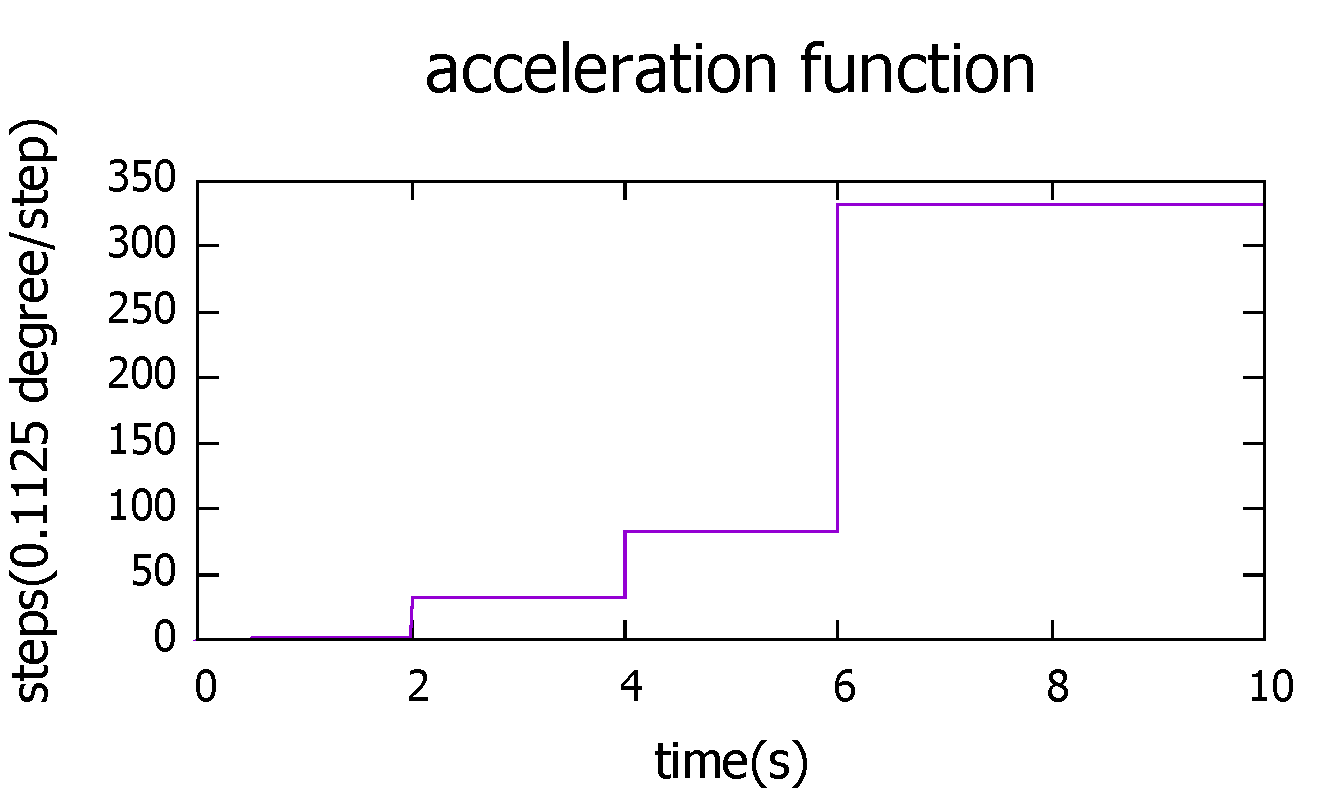
\includegraphics[width=0.9\linewidth, height=5cm]{function} 
		\caption{가속 기능}
		\label{fig:function}
	\end{subfigure}
	\begin{subfigure}{0.5\textwidth}
		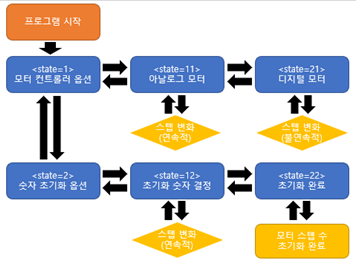
\includegraphics[width=0.9\linewidth, height=5cm]{algorithm}
		\caption{알고리즘}
		\label{fig:algorithm}
	\end{subfigure}
	\caption{펌웨어 설명}
	\label{fig:image3}
\end{figure}

\subsection{무선통신}

\subsubsection{블루투스}

\begin{wrapfigure}{l}{0.15\textwidth}
	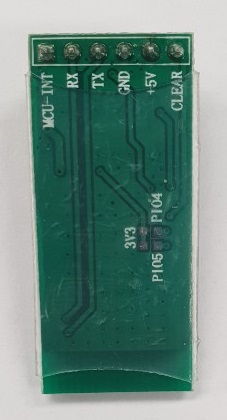
\includegraphics[width=1\linewidth]{HC06}
	\caption{HC06}
	\label{fig:HC06}
\end{wrapfigure}
블루투스는 보통 Arduino와 master-slave 관계를 맺어 정보를 서로 전달한다. OLED와 비슷하게 I2C 방식의 통신을 지원하는데, RX, TX 핀을 이용한 통신을 여러 가지를 실행하기 위해서는 “SoftwareSerial.h” 라이브러리를 이용하여 RX, TX 통신 핀을 여러 개로 따로 지정해주어야 한다.\\
본 연구에서 사용하는 모듈인 HC06 모델은 제품 스스로가 master가 될 수도 있고, slave로 설정될 수도 있다. (이와 비슷한 모델은 HC05는 slave 설정만 지원하기 때문에 아래에 서술할 방법을 사용하지 못함) 이를 발전시키면, 여러 개의 HC06을 활용하여서 한 모터 초점 조절 장치 컨트롤러에서 다른 모터 초점 조절 장치 컨트롤러로 정보를 서로 주고받을 수 있다.\\
블루투스는 페어링을 시키면 언제든지 사용할 수 있다는 장점이 있다.

\subsubsection{WIFI}

\begin{wrapfigure}{l}{0.06\textwidth}
	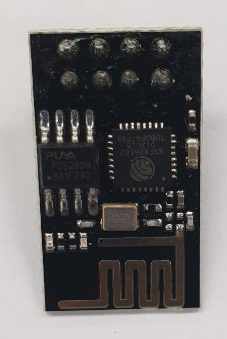
\includegraphics[width=1\linewidth]{ESP8266}
	\caption{ESP8266}
	\label{fig:ESP8266}
\end{wrapfigure}
가장 잘 알려져 있으며, 본 연구에서 사용하는 WIFI module인 ESP8266는 아두이노와 WIFI 연결을 가능하게 하여 준다. WIFI의 연결은 블루투스와 다르게 WIFI에 연결되어 있으면 언제든지 조절할 수 있다는 것이 큰 장점이며, IoT의 초기 모델로도 사용할 수 있다.\\
대부분의 WIFI module을 사용하려면 컴퓨터의 펌웨어를 업데이트해야 하므로 일반적으로 블루투스보다 사용이 어렵다. 

\subsection{ASCOM Protocol}

모터 초점 조절 장치를 활용하기 위해서는 별의 크기를 분석해서 돌려야 하므로 컴퓨터와의 연동을 위하여 초점 조절 장치의 ASCOM 드라이버를 C\# 코딩을 이용하여 제작한다. ASCOM 드라이버를 이용하면 카메라로부터 정보를 컴퓨터가 받아서 데이터를 분석하고, 이 분석한 데이터를 이용하여 모터를 어떻게 조절해야 할지 명령을 내리면 ASCOM 드라이버를 통해 정보를 전달하여 모터를 제어한 대로 조절이 가능하다.\\
현재 우리가 사용하는 프로그램은 ASCOM에서 만든 프로그램이고, ASCOM의 프로그램 대부분은 그 회사만의 표준 Protocol을 사용한다. 따라서 우리가 만드는 모터 초점 조절 장치 컨트롤러를 ASCOM Protocol에 따라 정보를 전달할 수 있도록 하면 일반 컴퓨터에 있는 ASCOM 프로그램을 이용하여 우리가 제작한 모터 초점 조절 장치 컨트롤러를 사용할 수 있도록 하는 것이 핵심이라고 할 수 있다. % 원래 있던 문
\section{결론}

 본 연구를 통하여 모터 초점 조절 장치 및 펌웨어 개발, 무선통신 개발, ASCOM 드라이버 개발 등을 통하여 자동 초점 조절 장치 개발을 위한 기반을 마련하였다. 이를 통하여 기존에 있던 초점 조절 장치의 성능을 무선통신 등의 여러 면으로 개선하여 사용자들에게 편의성을 제공하였다. 본 연구가 나아간다면 성능이 좋고 여러 가지 기능이 존재하는 자동 초점 조절 장치를 개발할 수 있을 것이다. 이와 관련된 자세한 내용은 이후 문서에서 다룬다.

\section{추후 연구}

\subsection{카메라(또는 CCD) 제어 Software 개발}

사진 관측을 이용해서 얻은 사진을 컴퓨터로 연결하여 분석이 가능할 수 있도록 만든 카메라(CCD) 제어 시스템을 개발한다. 이렇게 분석한 사진을 컴퓨터로 보낼 수 있어야 한다. 구체적으로 제어 시스템과 관련된 이야기를 하면, 카메라가 별의 크기와 관련된 정보를 분석해야 하는데, 이에는 두 가지 방법이 있다. 첫 번째 방법은 밝기의 기울기 값으로 초점이 맞음을 판단하는 것이다. 즉 수치화된 밝기를 이용하는 것이다. 각 픽셀에는 밝기에 대한 수치적인 정보가 존재한다. 인접한 픽셀의 수치 차이가 크다면 밝기 차이가 큰 것으로, 밝기 기울기가 큰 것이다. 이를 이용한다면 밝기 기울기가 가장 큰 순간이 초점이 맞았을 때로 판단하여 초점을 맞출 수 있을 것이다. 두 번째 방법은 천체의 크기로 초점이 맞음을 판단하는 것이다. 일정 밝기 이상의 픽셀에 대한 분포를 계산하는데, 각각 사진 중 가장 적은 픽셀이 조건을 만족하는 사진을 찾으면 그 사진을 초점이 맞았다고 판단할 수 있을 것이다. 이렇게 초점이 맞았음을 판단하는 것 외에도 카메라에 나오는 화면의 변화를 보아야 하므로 연속적인 변화를 실시간으로 보낼 수 있는 프로그램을 만들어서 컴퓨터가 제대로 인식을 하여 모터에 올바른 명령을 내릴 수 있는지 확인하면 가능하다.

\subsection{자동 초점 조절 알고리즘 구현}

천체망원경의 초점을 맞추기 위해 사진 관측의 사진을 연속적으로 찍어서 컴퓨터로 보내주고, 컴퓨터는 이를 분석하여 초점 조절 장치 컨트롤러에 별의 크기가 커지고 있는지 작아지고 있는지 정보를 알고리즘에 보내준다. 그러면 프로그래밍 된 Arduino가 모터를 어느 방향으로 돌려야 하는지 판단하여 모터를 돌리고, 이 과정을 반복하여 별의 초점이 맞을 때 이 과정을 멈춘다. 이러한 과정이 일어나는지 실제로 천체망원경으로 직접 확인하면 가능하다.

\subsection{추가 가능한 여러 가지 기능}

\subsubsection{STM32L432KC}

STM32L432KC는 ARDUINO NANO보다 성능이 좋은 Arduino로, 방향만 반대일 뿐 핀의 순서와 종류가 모두 같아 ARDUINO NANO에 넣었던 펌웨어를 그대로 사용할 수 있다.

\subsubsection{열선 설치}

날씨가 추운 날에는 모터가 얼어서 돌아가지 않거나 렌즈에 서리가 껴서 초점이 맞아도 맞지 않은 것으로 판단할 수 있다. 따라서 이를 예방하기 위하여 열선을 깔아서 DHT22에서 측정한 온도를 바탕으로 특정한 온도 이하로 내려가게 된다면 열선이 활성화될 수 있게 할 수 있다.

\subsubsection{PID 알고리즘}

PID는 보통 무엇인가를 제어하는 데 사용하는 일종의 ’제어 알고리즘’이다. PID 각각이 의미를 가지고 있는데, P는 제어, I는 적분, D는 미분 항의 세 가지를 가지고 있으며, INPUT이 존재할 시 이를 목표로 하는 목표점(setpoint)을 잡은 뒤, 이와 비교하여 오차를 계산하게 된다. 이 오차를 이용한 계산은 다시 목표점으로 부터의 오차를 구한 뒤 피드백 값을 이용하여 다시 제어에 활용을 하는 구조로 이루어져 있다.
PID의 각 역할을 다시 설명하자면, P(비례항)는 오차 값의 크기에 비례하는 제어작용, I(적분 항)은 오차를 줄이는 항이고, D(미분 항)는 출력 값의 급격한 변화를 늦추어 부드러운 변화형을 가질 수 있도록 한다.\\
PID 코드란 자신이 원하는 값에 빠르게 접근할 수 있도록 이용하는 코드이다. PID 코드를 이용하면 원하는 길이, 즉 초점이 맞는 길이에 부드럽고 빠르게 접근할 수 있도록 할 수 있으므로 시간 단축에 많은 도움이 될 것이다.

\subsubsection{EEPROM}

EEPROM은 Arduino 내부에 저장된 비휘발성 메모리로, 컴퓨터의 ‘RAM’과 같은 역할을 하고 있다. 비휘발성이기 때문에 Arduino를 초기화하거나 껐다가 다시 켰더라도 정보를 저장하고 있다.\\
Arduino별로 한 EEPROM의 주소에 들어갈 수 있는 수의 크기가 달라진다. ARDUINO NANO는 4KB의 EEPROM을 지원하므로 0~255까지의 수를 한 번에 저장할 수 있다. 이렇게 저장할 수 있는 수가 작으므로, 여러 가지 주소를 활용하여 큰 수 또한 나타낼 수 있다.(수를 진법으로 바꾸는 과정과 유사함)\\
실제로 이를 기반으로 펌웨어를 제작하여 보았지만, 수가 약 32000 이상으로 넘어가는 상황에서는 갑자기 수가 이상하게 커지는 오류가 발견되었고, 이를 고쳐야 할 것이다.

\subsubsection{모터의 연결 상태}

모터의 연결 상태는 펌웨어를 실행하는 데 아주 중요하다. 만약 펌웨어가 실행되는 도중에 모터가 연결되지 않으면, 스위치를 움직였을 때 스위치의 숫자는 움직이지만, 모터는 움직이지 않아 결과적으로 숫자의 오류를 불러일으킨다. 또한, 모터를 펌웨어가 실행되는 도중에 연결선을 뽑으면 펌웨어에 에러가 일어나는데, 이 경우 다시 모터를 꽂더라도 정상적으로 실행이 되지 않는다. 따라서 이런 여러 상황에 대하여 모터의 연결 상태를 대비한 에러 코드를 설정해야 숫자와 모터가 오차를 일으키는 일이 없을 것이다.


\bibliography{bibfile} % 참고문헌
% BibTeX 코드 쉽게 얻어오는 방법 %
% Google Scholar 에서 검색한 결과에서 `인용'을 클릭한다.
% BibTeX 코드를 얻고자 한다면, 하단의 `BibTeX' 을 클릭.
% 코드가 나온다. Ctrl+A, Ctrl+C로 복사, bibfile에 붙여넣기.


\end{document}
